%--------------------
% Packages
% -------------------
\documentclass[11pt,a4paper]{article}
\usepackage[utf8x]{inputenc}
\usepackage[T1]{fontenc}
%\usepackage{gentium}
\usepackage{mathptmx} % Use Times Font


\usepackage[pdftex]{graphicx} % Required for including pictures
\usepackage[danish]{babel} % Swedish translations
\usepackage[clean]{svg}
\usepackage[pdftex,linkcolor=black,pdfborder={0 0 0}]{hyperref} % Format links for pdf
\usepackage{calc} % To reset the counter in the document after title page
\usepackage{enumitem} % Includes lists

\frenchspacing % No double spacing between sentences
\linespread{1.2} % Set linespace
\usepackage[a4paper, lmargin=0.1666\paperwidth, rmargin=0.1666\paperwidth, tmargin=0.1111\paperheight, bmargin=0.1111\paperheight]{geometry} %margins
%\usepackage{parskip}

\usepackage[all]{nowidow} % Tries to remove widows
\usepackage[protrusion=true,expansion=true]{microtype} % Improves typography, load after fontpackage is selected

\usepackage{lipsum} % Used for inserting dummy 'Lorem ipsum' text into the template


%-----------------------
% Set pdf information and add title, fill in the fields
%-----------------------
\hypersetup{ 	
pdfsubject = {},
pdftitle = {},
pdfauthor = {}
}

%-----------------------
% Begin document
%-----------------------
\begin{document} 

\section{IsLeapYear algorithm}

\subsection{Algorithm description}
The algorithm is implemented by the method \textit{Calendar::IsLeapYear}. It takes a single parameter -- \texttt{year} of type \texttt{int}. The algorithm then has three \textit{guard clauses} and a default return value, that is stepped through as follows:

\begin{enumerate}[label=\textbf{Step \arabic*:}]
    \item If the input year is less than 1582, an exception of type \texttt{NotSupported} is thrown. The algorithm terminates.
    \item If the input year is not evenly divisible by 4, go to step 6. If it is, go to step 3.
    \item If the input year is evenly divisible by 100, go to step 4. If not, go to step 5.
    \item If the input year is not evenly divisible by 400, go to step 6. If it is, go step 5.
    \item The year is a leap year -- return true and terminate.
    \item The year is not a leap year -- return false and terminate.
\end{enumerate}
This is illustrated in a flowchart on the next page.
\newpage
\subsection{Diagram}
\begin{figure}[h!]
    \centering
    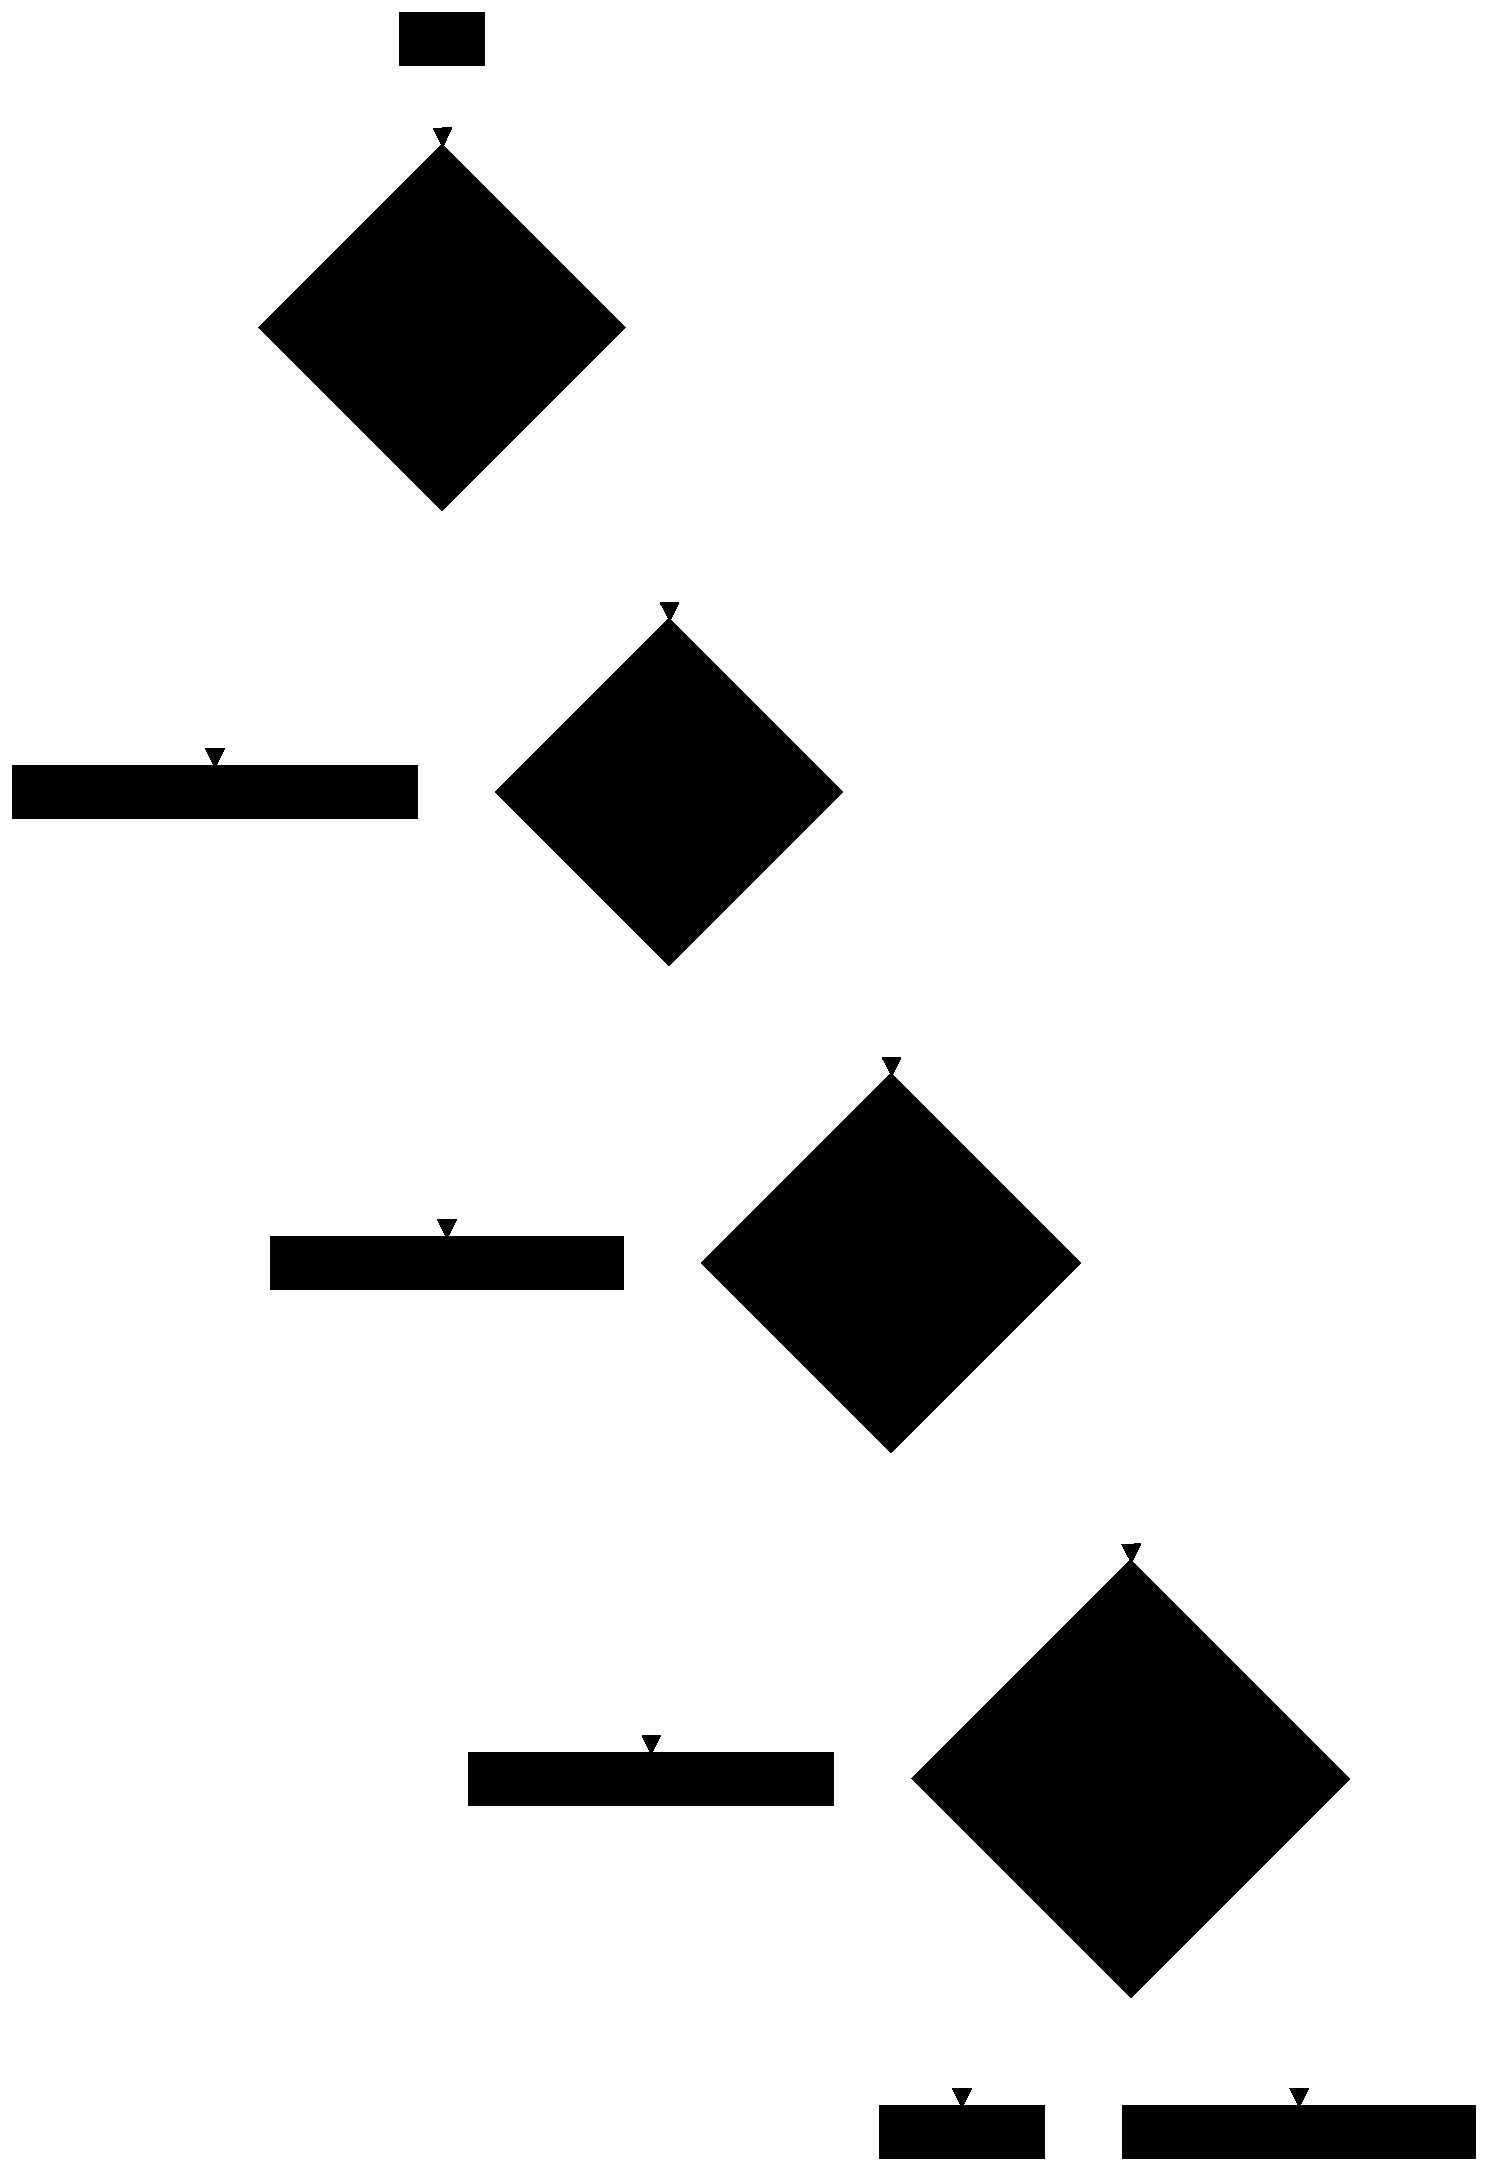
\includegraphics[width=0.95\linewidth]{diagram.png}
\end{figure}
\end{document}
